\chapter{Proposed Approach}
\label{chapter3}
Before describing the proposed approach we clarify the meaning of context, domain, usage, and GUI models. A domain model describes data, entities and their relationships in an application; it looks like a network of interconnected objects, where each object represents meaningful entities and concepts. Information in a domain model is useful to determine inputs and outputs in an application under test. A graphical user interface model (GUI) is also an informative model that represents all the graphic components and views of an application, and the events that trigger transitions among the views; it is commonly represented as a state diagram and it has been widely used for GUI ripping \cite{amalfitano_fasolino_tramontana_carmine_memon_2012}. A context model \cite{crashscope} represents the surrounding conditions in which an app runs; in the case of mobile applications, it also includes sensors, networking, available hardware information (\eg device model, processor version), screen resolution and O.S version. An usage model describes how users can interact with an application and what functionalities are offered to them \cite{monkeylab}.

By augmented model (or multi-model) we mean the combination of the aforementioned models, in a single model that synthesizes relevant information.  
%A top-down approach will be used to present our approximation to augmented models for Android apps. We propose to extract a context model, a domain model a GUI model and an usage model. Our starting point is an APK and a virtual o real device. The APK can be decompiled through reverse engineering tools (\eg APK Tool \cite{apkTool}) to do static code analysis. To dynamically explore the app, we propose automated installation of the APK into a device, followed by automated exploration through ripping strategies. 
More formally, a multi-model is a directed graph. $G = (V,A)$, with
$V $ a set of states, in which each state has a unique combination of contextual variables,  GUI elements and domain entities; and 
$A$ a set of transitions, where each transition is a contextual change in the APP or an user interaction in the GUI that triggers a change in the app to a new state.

We illustrate the multi-model concept with the example presented in \figref{multimodel}; the Figure depicts an abstraction for a multi-model  generated dynamically and statically from a test app developed by the authors. The multi-model  has 3 states (\textit{S1}, \textit{S2} and \textit{S3}), and 2 edges (\textit{T1} and \textit{T2}). In this example, the app is impacted by contextual changes. %Turning off Wi-Fi in the home screen activates an alert dialog (S3) that warns the user about using bluetooth because Wi-Fi is off.  Otherwise, clicking a button in the home screen (S1) changes the app to a state where a domain element can be created by filling a text box (S2). In this scenario, a multi-model is representing a complete abstraction with domain, GUI, context and usage elements.

\begin{figure}[t]
	\centering
	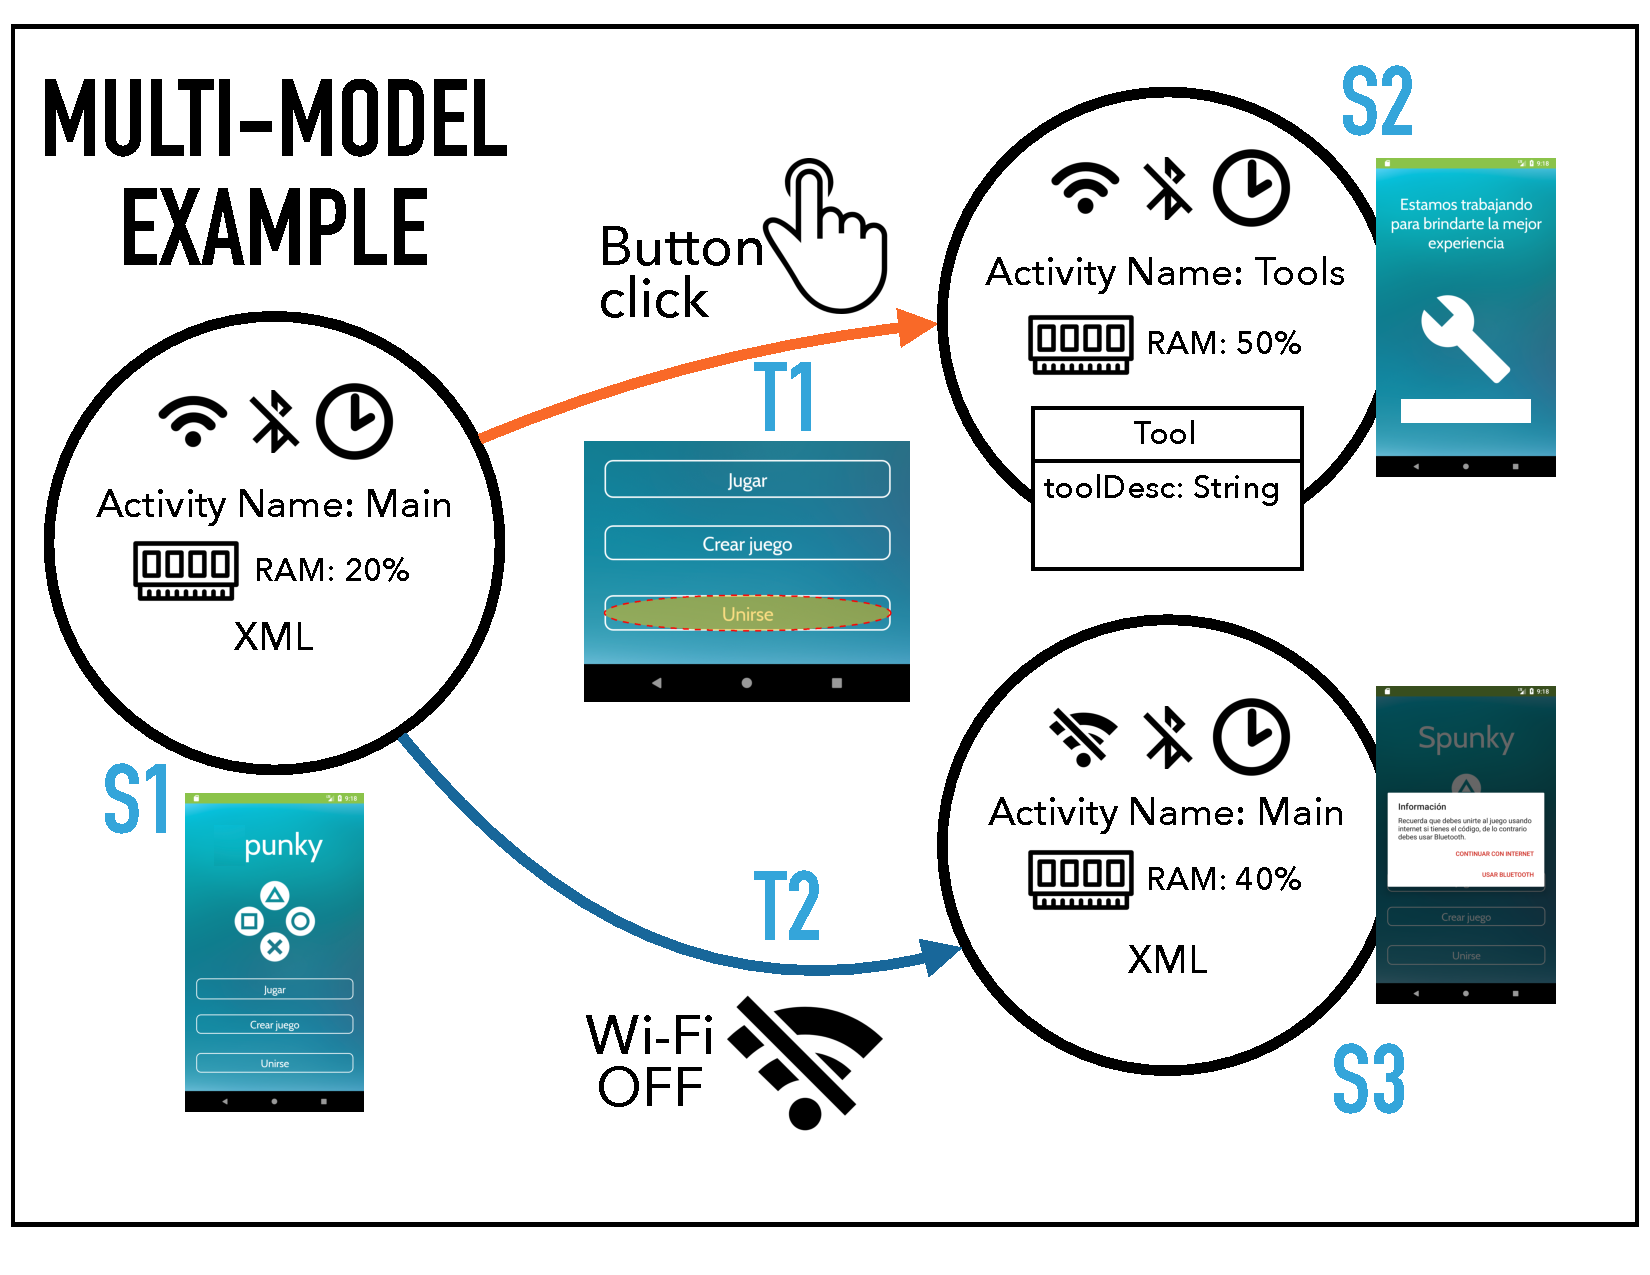
\includegraphics[width=1\textwidth]{img/multimodel.pdf}
	\vspace{-0.8cm}
	\caption{Example of multi-model generated from an Android app. The states and transitions are a subset of the complete multi-model for the analyzed app.}
	
	\label{multimodel}
\end{figure} 


\textit{S1} is the home window of the application. It is a state that mixes graphical, usage and context information. \textit{S1} occurs when Wi-Fi and cellular networks are active. On average, when this state is  active, the device has an availability of 80\% of its memory. %\textit{S1} also contains a XML screenshot of its graphical layout and an image.  
From \textit{S1}, the app flow can go to two states (\textit{S2} and \textit{S3}). The transition from \textit{S1} to \textit{S3} (\textit{T2}) occurs when Wi-Fi is turned off. \textit{S3} is a state running the same activity as \textit{S1}, however, it displays an alert message that fades out other buttons and the background. \textit{S3} is more memory greedy than the initial state.

Transition \textit{T1} changes app state from \textit{S1} to \textit{S2}. This transition is activated by clicking the button located at the bottom of the screen. Once this button is pressed, \textit{S2} is activated.  Context, graphical and usage information is also available in \textit{S2}, however, it also includes domain-related information because there is a text-input for collecting information from the user; thus, we consider the activity (\ie the Android window related to \textit{S2}) as an entity named ``Tool” with a string field called ``toolDesc”.

%Summarizing \figref{multimodel}, this example app with 3 states is affected by contextual changes. Turning off Wi-Fi in the home screen activates an alert dialog. When this alert appears, more RAM memory is being used in the device. Clicking a button in the home screen changes te app to a state where a domain element is created by filling a text box. In this scenario, a multi-model is representing a complete abstraction with domain, GUI, context and usage elements.

\section{General Approach}

\begin{figure}[t]
	\centering
	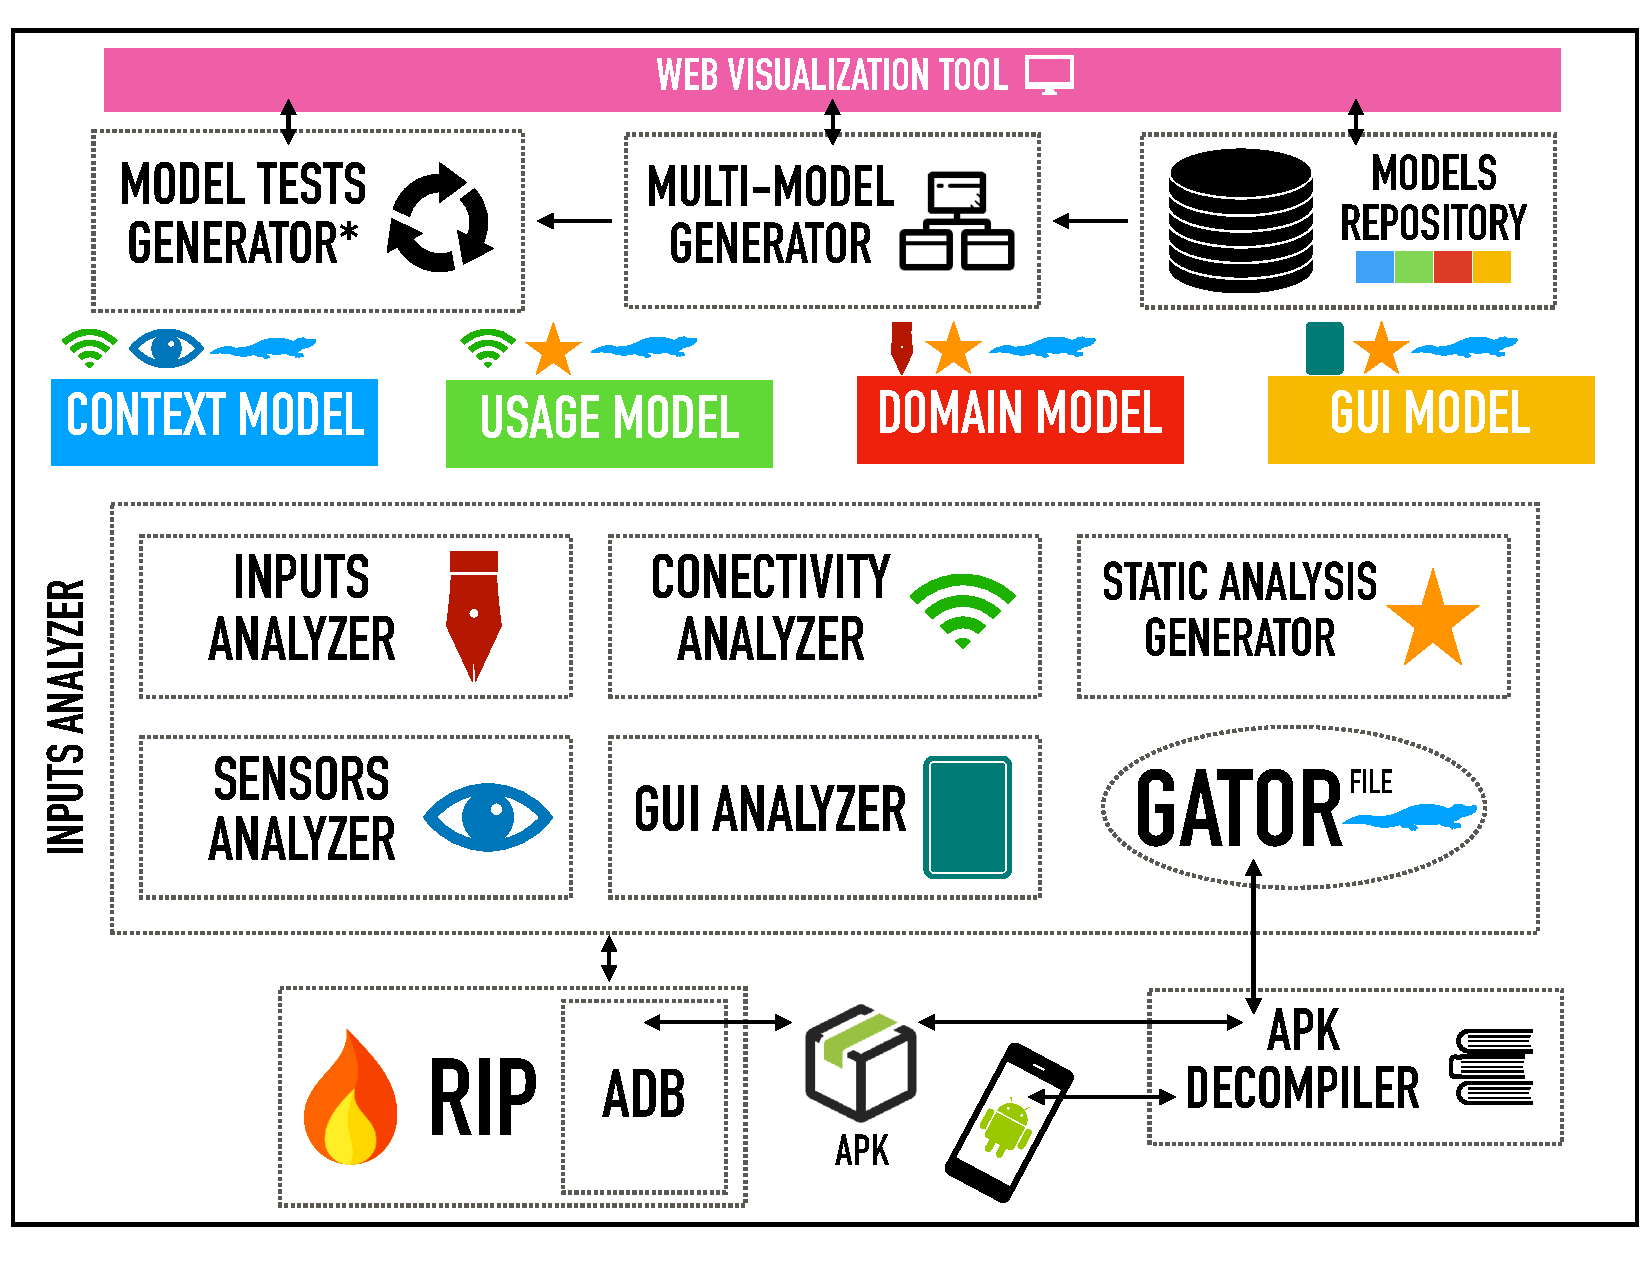
\includegraphics[width=1\textwidth]{img/generalArchitecture.pdf}
	\vspace{-0.8cm}
	\caption{Proposed architecture (\textbf{RIP}) for extracting augmented models for Android apps.}
	\label{generalArchitecture}
\end{figure}	

We have designed an  architecture \figref{generalArchitecture} that enables a series of stages that include: ripping, automatic extraction of static and dynamic models, generation of multi-models and model-based tests generation.

The multi-model generation starts by ripping the app under test. For this purpose, we have designed and developed a desktop tool called \textbf{RIP}, which is publicly available at \url{https://github.com/TheSoftwareDesignLab/rip}. It is an automation software that executes a series of actions and emulates user interactions into an Android device to extract models; this is done through the Android Debug Bridge (ADB) \cite{adb}, a command-line tool that provides access to an Android device over USB or Wi-Fi. In comparison to monkey/random testing tools that generate random interactions to find bugs and corner cases, \textbf{RIP} follows an strategy to explore the application based on the dynamic content that appears on a device screen (like other rippers do). \textbf{RIP} not only simulates user interactions in the screen; \textbf{RIP} also executes contextual changes to the application that vary the network configuration and the readings of the sensors (\eg accelerometer, gravity, gyroscope, light, proximity, magnetic field).  During the execution,  \textbf{RIP} collects GUI-related, domain-related. sensors-related, and resources-related information. In addition, screenshots and  GUI-hierarchies are collected for each state.

Our approach differs from existing ones because we are able to (i) generate a comprehensive list of contextual changes, (ii) extract a domain model from GUI states,  (iii) augment the dynamically-generated model with information collected statically, and (iv) considers exploration of hybrid applications. Due to security restrictions imposed by Android devices and the Android framework, in order to enable contextual events execution via ADB (\eg airplane mode, Wi-Fi), it is necessary to run the commands in a rooted physical device or an emulator.

\textbf{RIP} takes advantage of static code analysis to enrich the final generated model. When the ripping process finishes, RIP augments the collected model with a graph generated statically by GATOR \cite{gator}, a static reference analyzer tool for GUI objects in Android. This tool has been chosen because its context-aware approach in static code analysis \cite{yang_yan_wu_wang_rountev_2015}. GATOR finds static references to GUI components and determines its control flow. If \textbf{RIP} identifies missing states (\ie states detected by GATOR but not by \textbf{RIP}), it adds the new states to the dynamically generated model. Thus, the  GUI and usage models are represented by the combination of transitions and states information extracted from the ripping and GATOR.

GATOR code is not included in \textbf{RIP}. To combine static information with RIP's execution, GATOR analysis should be run first, and then passed to \textbf{RIP}. An example of the file that \textbf{RIP} imports from GATOR is presented in the code example \ref{gatorFile}

\begin{lstlisting}[language=json, caption={Fragment of a GATOR file obtained from a native application}, label={gatorFile}, firstnumber=1]
{ "nodes": [{
"id": 2160,
"name": "com.simplemobiletools.commons.activities.FAQActivity"
}, {
"id": 2076,
"name": "android.view.Menu"
}, {
"id": 2140,
"name": "android.view.Menu"
}, {
"id": 14106,
"name": "android.app.DatePickerDialog"
}],
"edges": [{
"source": 2076,
"target": 2140,
"event": "implicit_power_event"
}, {
"source": 14106,
"target": 14106,
"event": "implicit_home_event"
}, {
"source": 2140,
"target": 2140,
"event": "implicit_rotate_event"
}, {
"source": 2160,
"target": 2160,
"event": "implicit_home_event"
}]}
\end{lstlisting}

\section{RIP components}		

Our architecture defines a layer of analyzers that guide \textbf{RIP} during the models extraction:

\subsection{GUI analyzer}

It extracts the hierarchy of graphical components in the app. It is able to differentiate app GUI states based on the analysis of the GUI hierarchy represented as an XML file. It means, the construction of the GUI model is done iteratively, according to the app exploration. To determine if two views are different, a decision process is followed. Firstly, if the activity names differ from each other, the two views are classified as different states. Otherwise, if the activity names are the same, then the XML is analyzed; each view is compared by the number of elements, checked boxes,  buttons, labels content, alerts, and messages.  In the case of menus or dialogs that are displayed on a view, we consider them also as states.

\begin{lstlisting}[language=xml, caption={XML dump from an app, containing the layout hierarchy},label={xmlDump}]
<?xml version='1.0' encoding='UTF-8' standalone='yes' ?>
<hierarchy rotation="0">
<node index="0" text="" resource-id="" class="android.widget.FrameLayout" package="com.clockwork.mcdonalds"
content-desc="" checkable="false" checked="false" clickable="false" enabled="true" focusable="false" focused="false"
scrollable="false" long-clickable="false" password="false" selected="false" bounds="[0,0][1080,1794]">
<node index="0" text="" resource-id="" class="android.widget.LinearLayout" package="com.clockwork.mcdonalds"
content-desc="" checkable="false" checked="false" clickable="false" enabled="true" focusable="false"
focused="false" scrollable="false" long-clickable="false" password="false" selected="false" bounds="[0,0][1080,1794]">
<node index="0" text="" resource-id="android:id/content" class="android.widget.FrameLayout" package="com.clockwork.mcdonalds"
content-desc="" checkable="false" checked="false" clickable="false" enabled="true" focusable="false"
focused="false" scrollable="false" long-clickable="false" password="false" selected="false" bounds="[0,63][1080,1794]">
<node index="0" text="" resource-id="" class="android.widget.ImageView" package="com.clockwork.mcdonalds"
content-desc="" checkable="false" checked="false" clickable="false" enabled="true" focusable="false"
focused="false" scrollable="false" long-clickable="false" password="false" selected="false" bounds="[0,63][1080,1794]" />
</node>
</node>
<node index="1" text="" resource-id="android:id/statusBarBackground" class="android.view.View" package="com.clockwork.mcdonalds"
content-desc="" checkable="false" checked="false" clickable="false" enabled="true" focusable="false"
focused="false" scrollable="false" long-clickable="false" password="false" selected="false" bounds="[0,0][1080,63]" />
</node>
</hierarchy>
\end{lstlisting}

%Some thresholds can be configured by the developer to change the sensitivity of states detection. 

The set of states gathered from visual information are the source for the GUI model. \textbf{RIP} captures image screen-shots and  XML layouts from every state it has found. It also records the interaction/event that triggered the state transition (\eg pressing a button); note that state transitions are modeled as edges connecting states. To extract the XML layout information, \textbf{RIP} executes the command \verb|adb shell uiautomator dump|. Eventually, the device stores this dump into an XML file such as the code example \ref{xmlDump}. Because this file is stored in the SD card, it must be extracted and parsed in the host computer. To capture the image snapshot of the device, a remote screen-shot is invoked with the command \verb|adb shell screencap|. All the files in the devices are extracted through \verb|adb pull|.

%The GUI model finally will be shown as a state diagram, including transition as edges connecting different states of the application.


\subsection{Inputs analyzer}

It enables \textbf{RIP} to identify user input-related GUI Android components and interact with them accordingly (\eg check boxes, text boxes, lists, scrollable views).  \textbf{RIP} creates random input data for the components based on the input types defined for text fields, and the component nature (\eg a check box can be activated or deactivated). Keyboards that appear on the screen and GUI components meta-data, give us clues about concepts and domain entities that are part of the domain model of the application. 
We define entities of the domain model as views that have input elements. Each entity has a set of attributes that correspond to input-related components in the view, and the attributes type is inferred from the type of input allowed (\eg numbers, special characters, boolean check, lists, \etc). 

\subsection{Sensors analyzer}

During the ripping, \textbf{RIP}  turns off/on sensors, randomly. The sensors analyzer identifies which sensors the application has access to from the app's manifest file. Once the sensors analyzer has this information, it detects the states where sensors are on and off using specific ADB commands. 

To obtain a detailed list of sensors, \textbf{RIP} invokes the command \texttt {adb shell pm list features}. The available sensors in the device are listed as features (\eg \verb|hardware.camera|,  \verb|hardware.sensor.gyroscope|, \verb|hardware.sensor.light|)

\subsection{Connectivity analyzer}

This component identifies connectivity status of the app during all the ripping execution. Once the GUI has detected an initial set of states, it sends requests to the device in order to control Bluetooth, Wi-Fi, celullar networks and airplane mode. \textbf{RIP} triggers connectivity changes in every view of the application. If an error occurs or the GUI changes after the contextual change, then a new state is  discovered and added to the model.

To determine the connectivity settings of the device, \textbf{RIP} calls the command \texttt {adb shell dumpsys wifi | grep 'Wi-Fi is'} to determine Wi-Fi status, \texttt {adb shell dumpsys wifi | grep 'mAirplaneModeOn'} to determine Airplane Mode, etc. The activation or deactivation of these settings is done with the commands  \texttt {adb shell svc wifi (disable|enable)}, \texttt {adb shell svc bluetooth (disable|enable)}, \texttt {adb shell svc data (disable|enable)}, etc. Commands that enable or disable connectivity settings of the device require root privileges.


\subsection{Static analyzer and GATOR}
Different from the other components, it imports a flow graph of the app based strictly on static analysis, by relying on the GATOR tool \cite{gator}. GATOR creates a window transition graph with activities, dialogs and menus. The transitions of the graphs include events such as button pressings and window stack operations (push and pop). This flow graph is used to augment the model collected dynamically by  \textbf{RIP}, in particular to have a more comprehensive list of transitions and states. This graph is presented in the code example \ref{gatorFile}.

%	\begin{figure}[h]
%		\centering
%		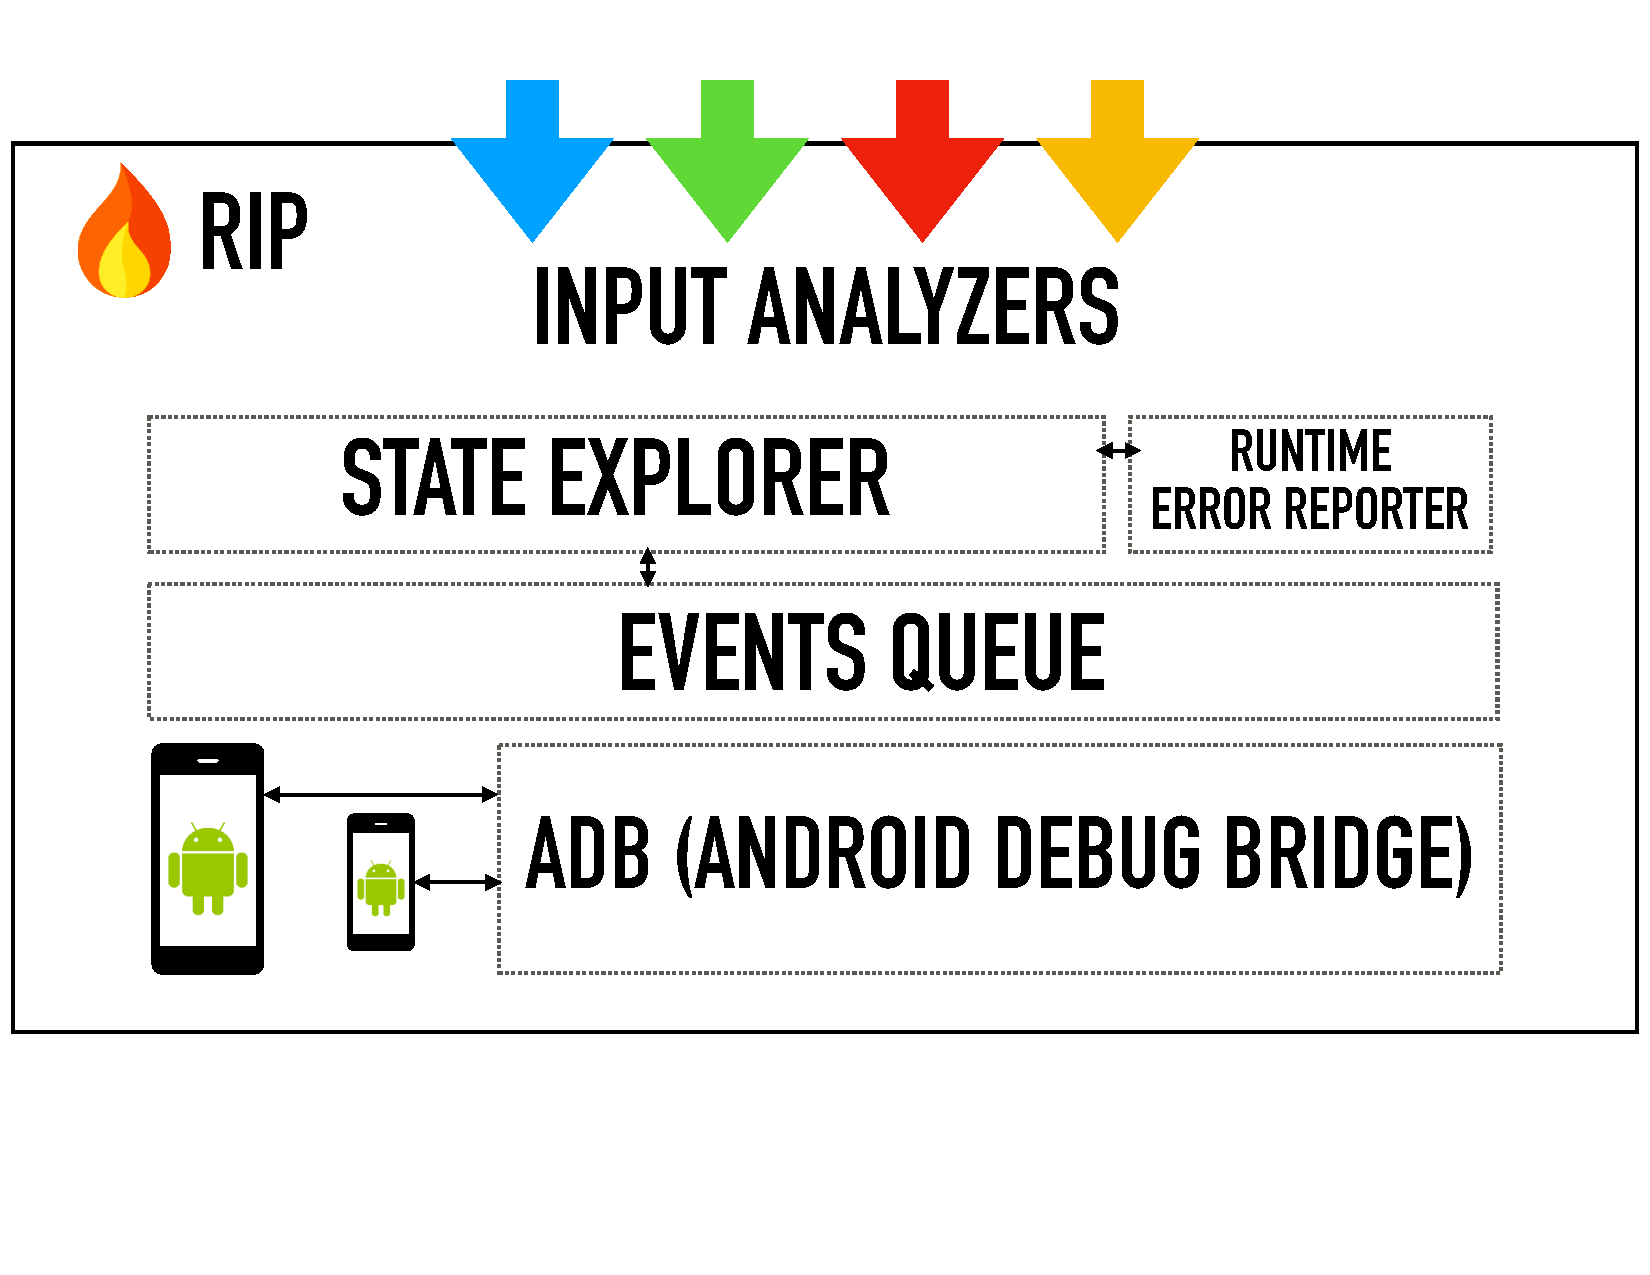
\includegraphics[width=0.5\textwidth]{img/ripArchitecture.pdf}
%		\caption{RIP components.}
%		\label{ripArchitecture}
%	\end{figure} 
%	

\subsection {RIP GUI}
It interacts directly with ADB to explore the applications dynamically and coordinates the execution of the other components. The \textbf{RIP} GUI combines the ripping, interactive data collection, and static analysis, to generate individual models and a multi-model like the one presented in \figref{real}; the \textbf{RIP} GUI also generates the model as a JSON file that can be analyzed by any other tool.

%\textbf{RIP} identifies native graphical Android elements to explore systematically every possible view of the app. This tool is able to simulate user interactions and contextual changes. RIP sends the gathered information to all the analyzers in order to build the mentioned models. \figref{real} presents a multi-model generated from our test app.

\begin{figure}[t]
	\centering
	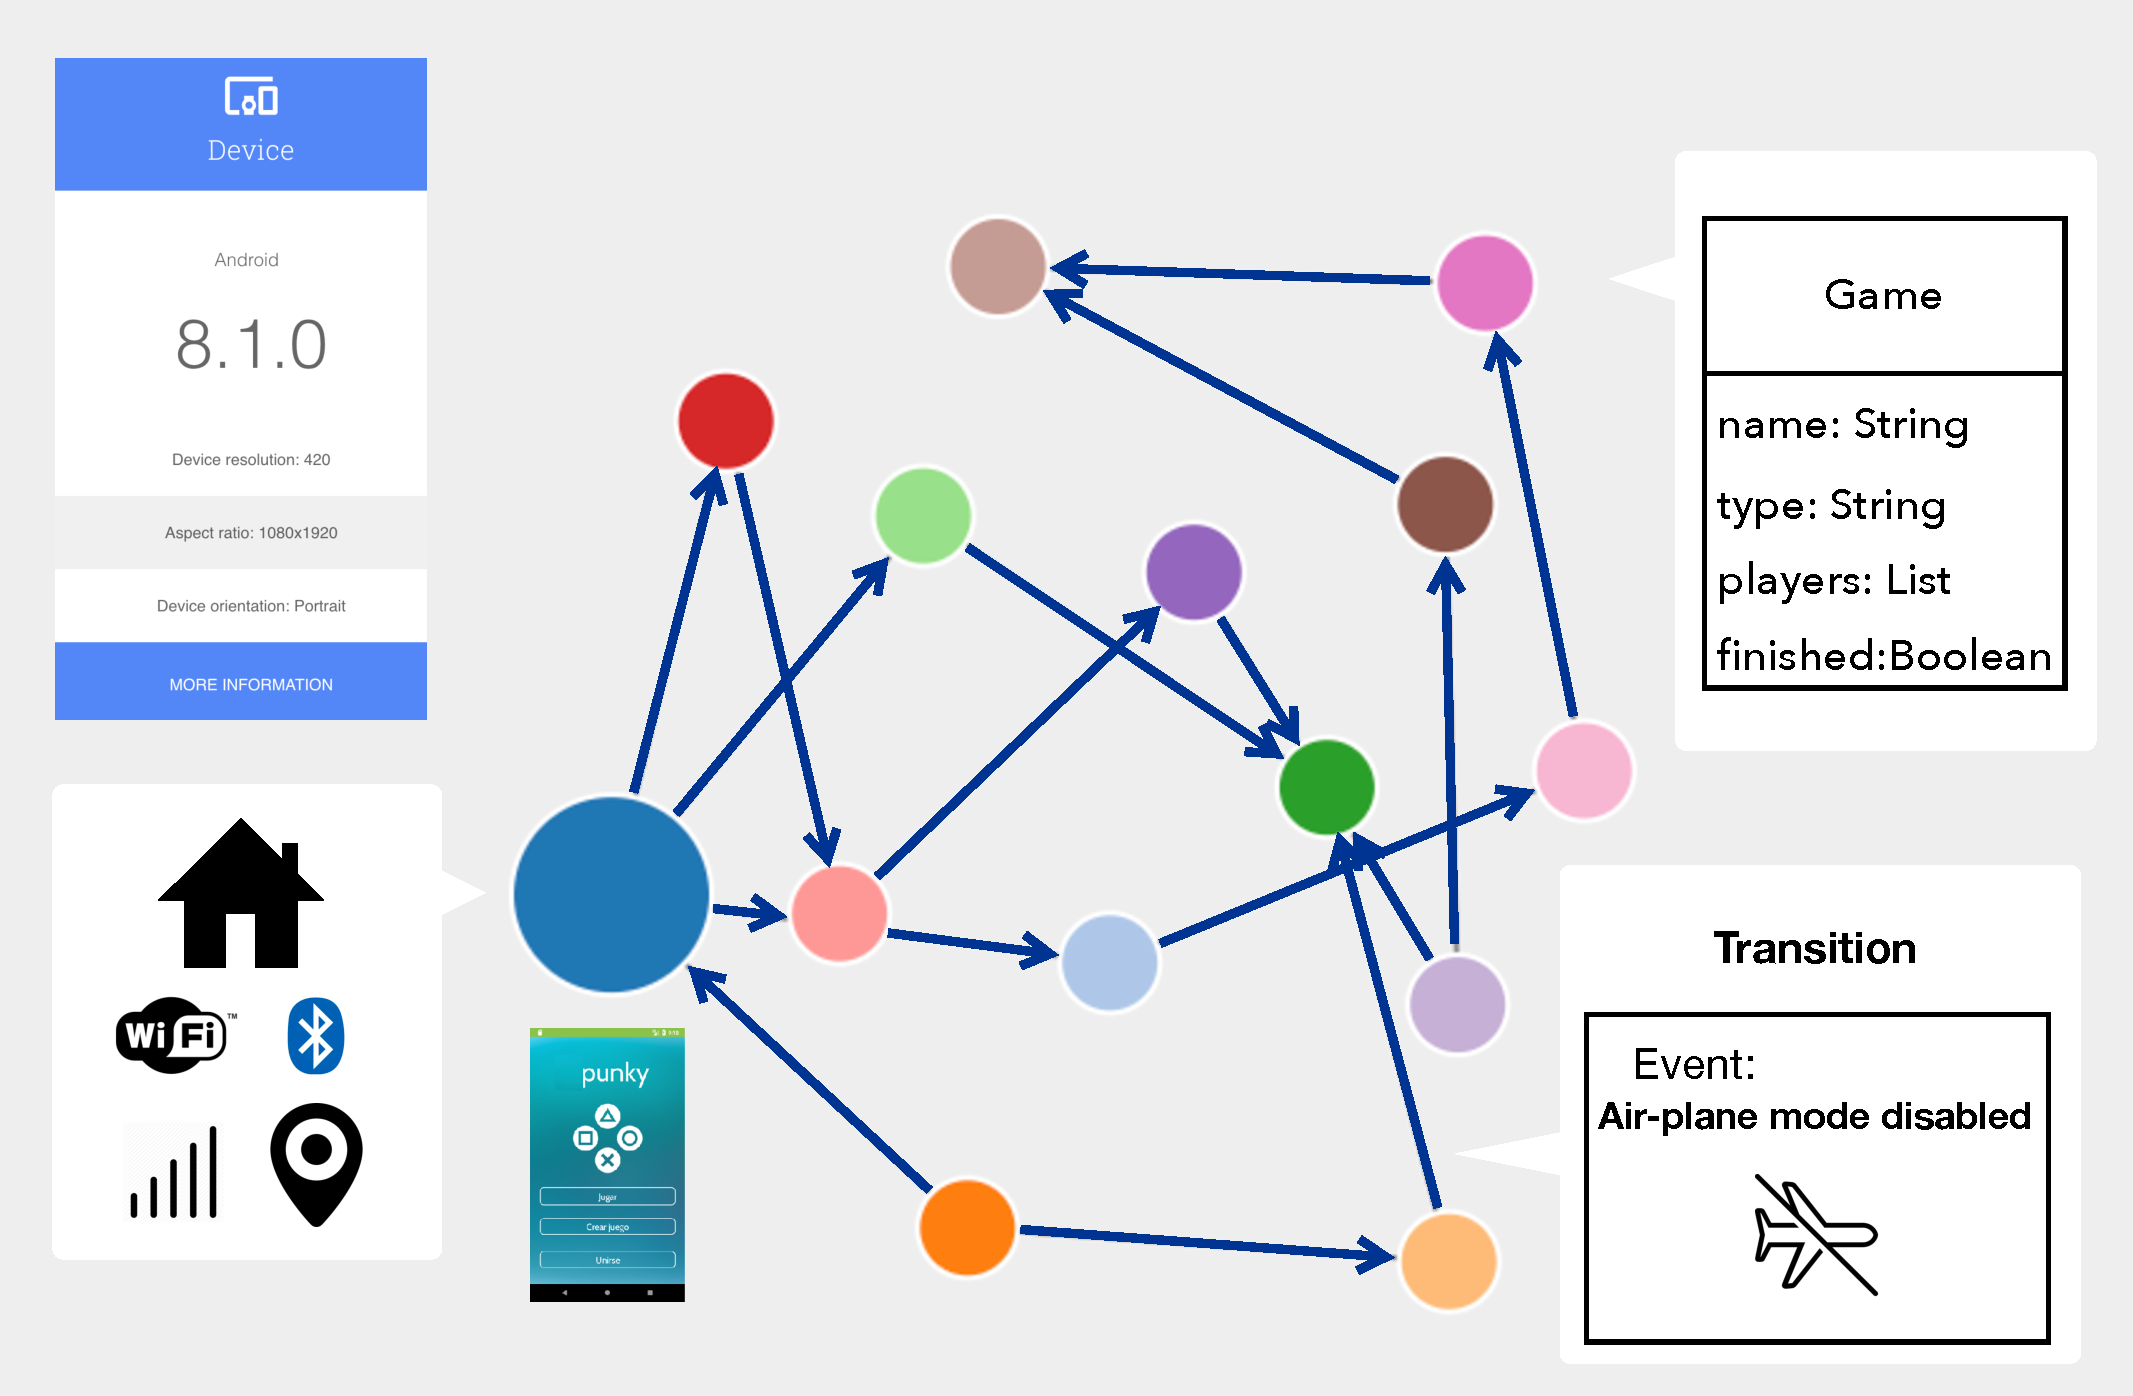
\includegraphics[width=1\textwidth]{img/multimodel-real.pdf}
	\vspace{-0.8cm}
	\caption{Example of multi-model created by RIP.}
	\label{real}
\end{figure} 

%	RIP general architecture is presented in \figref{ripArchitecture}. RIP communication with the device is done through Android Debug Bridge (ADB).
%	
%	\subsubsection{Events Queue}
%	RIP has an events queue that manages and synchronizes events between ADB and the state explorer. 
%	
%	\subsubsection{State explorer}
%	The states explorer is the controller of the automated interactions against an application. Once an APK is installed in a device, it defines the exploration strategy that RIP will follow. Input analyzers send request to the state explorer to push and pull information from the headset.
%	
%	Exploration could follow two principles. First, random exploration introduces random interactions into the app. These interactions include GUI analyzer interactions (\eg pressing random buttons, selecting check boxes, swiping), Input analyzer interactions(\eg Introducing text strings, numbers), connectivity interactions (\eg enable airplane mode, disable Bluetooth) and sensors interactions (\eg simulate a move of the accelerometer). This exploration method can be executed until a number of interactions have been done or until a timer ends.
%	
%	Second principle of exploration is guided exploration. It includes the same interactions, but this time it sets itself the objective of explore and cover the maximum amount of possible states. This kind of exploration is done by DFS and request the analyzers to create all the possible configurations for each view changing connectivity and sensors informations.
%	
%	\subsection{ Models repository}
%	
%	Models repository condenses all the generated models to be processed by the multi-model generator.
%	
%	\subsection{Multi-model generator}
%	
%	The multi-model generator takes as input the context, usage, domain and GUI models and combines all the models into a richer sate diagram.
%	
%	%\subsection{Test generator}
%	
%	%Test generator is currently not developed, however, it is a future step that will enable model-based testing based on the multi-model generation.
%	
%    \subsection{WEB visualization tool}
%    
%    Finally, a web visualization tool based on Javascript, HTML and D3 presents the final  multi-model. All the intermediate models are also included. This tools is presented in \figref{webTool}.
%    
%    \begin{figure}[h]
%    	\centering
%    	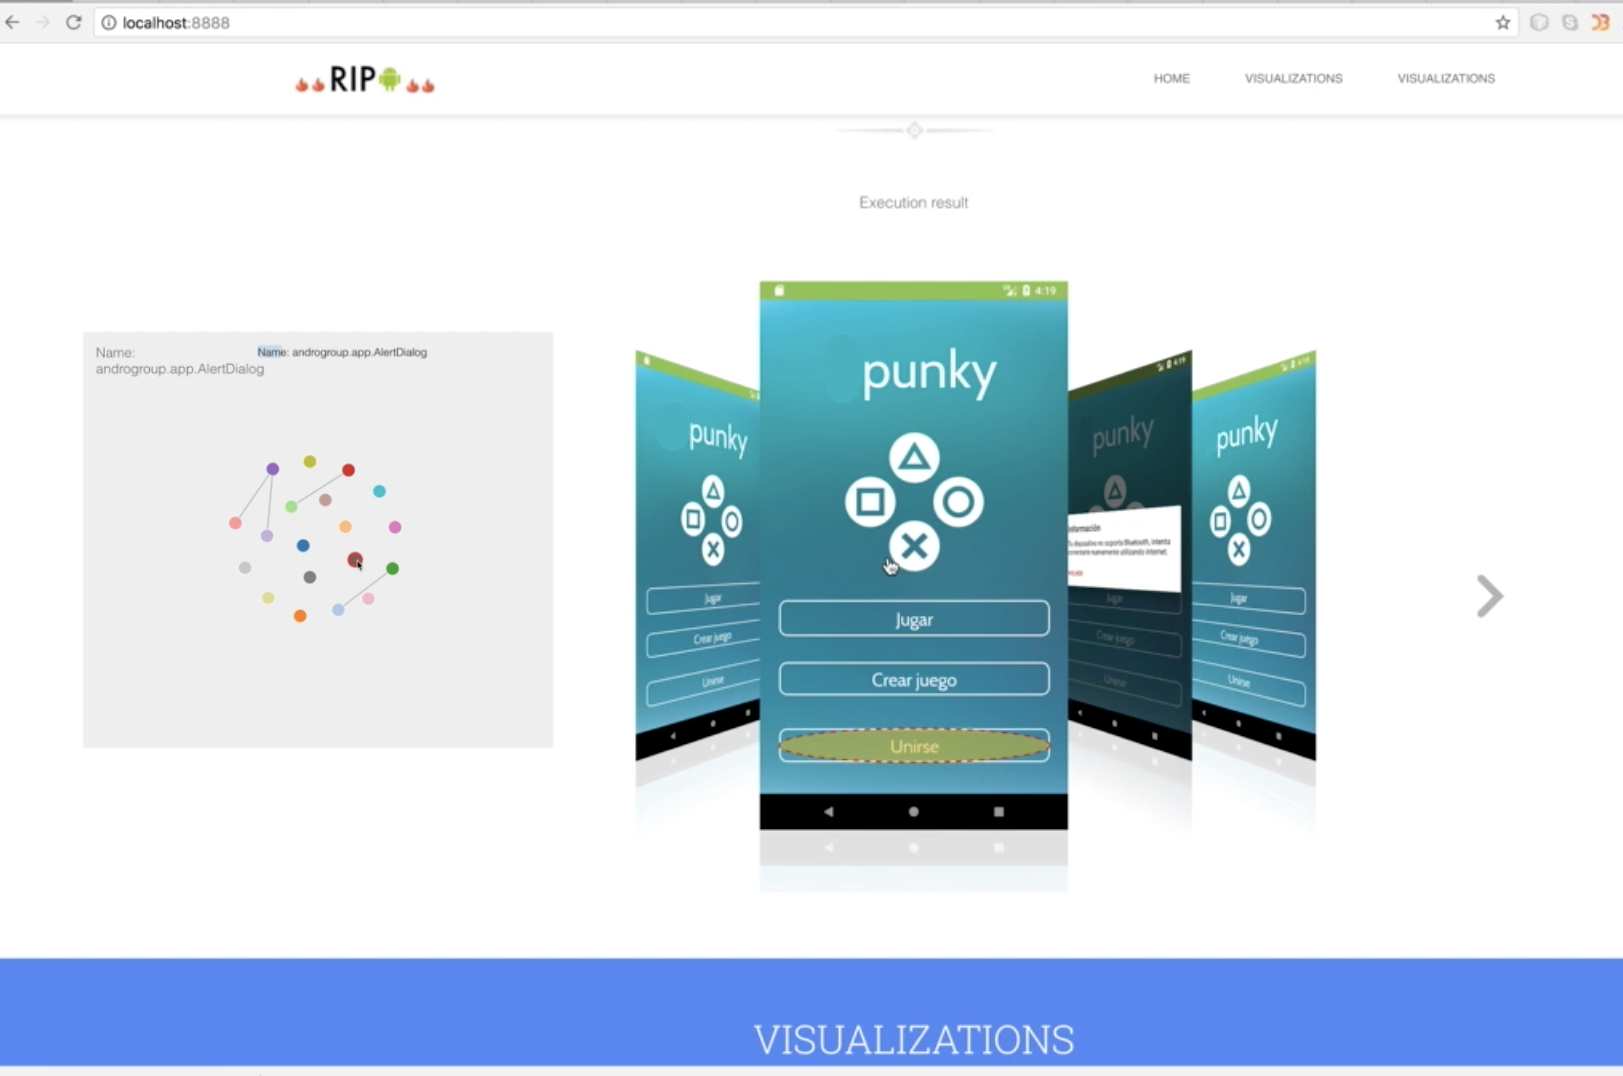
\includegraphics[width=0.5\textwidth]{img/webTool.png}
%    	\caption{WEB visualization tool}
%    	\label{webTool}
%    \end{figure} 

\section{Ripping  hybrid applications}
As described before, hybrid apps are those in which developers write significant portions of their application in cross-platform web technologies, while maintaining direct access to native APIs when required \cite{ibmHybrid}. This way of developing applications is gaining popularity among the mobile developers community because:
\begin{itemize}
	\item Reduces the time to develop cross platform apps
	\item It is based on Web technologies, which allows developers to recycle modules and components from existing Web developments
	\item Browser engines are becoming faster and mobile devices more powerful
	\item Performance differences between native and web technologies are becoming imperceptible
\end{itemize}

Currently, Apache Cordova is the component that enables the access to native iOS and Android APIs from the JS code. This piece of software gives access to Local Storage, Camera, GPS, and all the available sensors of each platform. Apache Cordova is the core of many popular hybrid frameworks such as Ionic, Adobe Phonegap, Monaca or Visual Studio. 

\subsection{Barriers for ripping hybrid apps }
Ripping native apps is different from ripping hybrid apps. The main reason is the underlying techonologies; in native apps the GUI is rendered by the view system and window manager of the  framework, in hybrid apps the GUI and events are managed by a Web View. In native applications, a native layout defines the structure of the user interface. An activity contains a hierarchy of containers and graphical objects called \textit{Views} and \textit{View groups}. These objects are also known as \textit{widgets}. Widgets could be instanced as elements such as buttons, labels, text fields, among others. View groups provide the structure of widgets and other view groups in the screen \cite{layouts}. To crawl dynamically apps, this hierarchy must be extracted continuously, and based on the layout information, the ripper can execute commands and simulate user interactions.

Contrary to native applications, most hybrid applications contain just one activity. This activity has a basic layout with a central element: a \textit{Web view} \cite{webView}. Web views are widgets that can render web content \figref{hybridCordova}. When the user interacts with elements of the web view, the JavaScript engine is in charge of changing the view. All the application logic is entirely written in JavaScript, therefore, errors, bugs and crashes are only visible to the web console. Additionally, the HTML DOM is not visible through the \verb|adb dumpsys| command.

\subsection{Strategies for ripping hybrid apps }
In \textbf{RIP}, we have defined and implemented a series of strategies designed to tackle the ripping of hybrid apps. Specifically, we consider important to maximize the coverage of states discovered and enable detection of crashes, while maintaining the  strategy of multi-model extraction and contextual exploration. 

\subsubsection{Detecting crashes in hybrid apps}
Crashes are usually the result of uncaught exceptions. Other crashes come from ANRs (\textit{Application Not Responding}), permission denials, network errors, and bad practices. These kind of crashes are well defined in the Android Developers Documentation and if one of them occurs, it is reported in the device. When one of these crashes is thrown, rippers of native apps are able to recognize them because the device writes them in the device log (logcat). In general, hybrid applications do not deal with these errors as native applications do, because their errors  are written in the JS console. In order to capture errors in hybrid applications, RIP reads continuously the WebView console with the help of Chromium.

While \textbf{RIP} crawls a hybrid application, it listens to the web console, and stores the web errors associated with each state. As these errors occur in an embedded web browser, all the HTTP errors can be associated to the running application. %As an example, in Figure \ref{hybridError} is depicted a 503 HTTP status code: Service unavailable.

\subsubsection{Maximize the coverage of states discovered}
In order to maximize the coverage of states discovered, \textbf{RIP} must interact with every 'clickable' element inside the web view. The exploration should not be focused on finding and interacting with Android widgets, but with every new component accessible in the web view. A better approximation to explore the hybrid GUI should extract and parse the DOM of the web components with the help of the Chrome inspector, however, this is considered as future work.

We found experimentally that introducing some randomness to the ripping process in these applications improves the discovering of new states, because not all the web elements can be extracted solely with UIAutomator, and always remains actions of the application that could not be accessed systematically.

Finally, a key step that improves exploration of hybrid apps is triggering contextual changes, specifically, toggling network and Internet settings. This occurs because sometimes, all the web view content is not served just from the mobile device, but also from external servers in the Internet. Hybrid applications are highly prone to errors due to contextual changes.

\begin{lstlisting}[caption={Pseudocode describing the Ripping process},label={pseudocode}]
transitions = []
discoveredStates = []
contextualChanges = [rotateScreen, turnOnWifi, ...]
func explore(t):
	s.clickOrExecute()
	transitions.push(s)
	if thisIsANewState():
		discoveredStates.push(currentState)
	if state.hasClickableElementsLeft():
 		for everyClickableElementInState c:
     		if c has not been clicked:
         		explore(c)
 	elif !state.hasClickableElementsLeft() and !state.contextualChangesDone():
 		for every cc in contextualChanges:
 			explore(cc)
 	elif state.ContextualChangesDone()
 		if state.isHybrid():
 		 	enableJSConsole()
 			action = randomAcctions()
 			explore(action)

\end{lstlisting}

